% IEEE standard conference template; to be used with:
%   spconf.sty  - LaTeX style file, and
%   IEEEbib.bst - IEEE bibliography style file.
% --------------------------------------------------------------------------

\documentclass[letterpaper]{article}
\usepackage{spconf,amsmath,amssymb,graphicx}
\usepackage{algorithm}  
\usepackage{algorithmic}
\usepackage{blindtext} %package to use \blindtext
\usepackage{hyperref}
\usepackage{soul}
\usepackage{enumitem} %simple interface to customize the appearance of lists

\renewcommand{\algorithmicrequire}{\textbf{Input:}}  % Use Input in the format of Algorithm  
\renewcommand{\algorithmicensure}{\textbf{Output:}} % Use Output in the format of Algorithm  
\newcommand{\RomanNumeralCaps}[1]
    {\MakeUppercase{\romannumeral #1}}
\def\sn#1{{\footnotesize\textbf{[SN: #1]}}}
% Example definitions.
% --------------------
% nice symbols for real and complex numbers
\newcommand{\R}[0]{\mathbb{R}}
\newcommand{\C}[0]{\mathbb{C}}

% bold paragraph titles
\newcommand{\mypar}[1]{{\bf #1.}}

%in order to highlight parts of pseudocode
\usepackage{minted}

% Title.
% ------
\title{Optimization of an Improved SPH Simulator}
%
% Single address.
% ---------------
\name{Silvia Nauer, Mengdi Wang, Tianwei Yu and Valérie Kulka}
\address{Department of Computer Science\\ ETH Zurich, Switzerland}

% For example:
% ------------
%\address{School\\
%		 Department\\
%		 Address}
%
% Two addresses (uncomment and modify for two-address case).
% ----------------------------------------------------------
%\twoauthors
%  {A. Author-one, B. Author-two\sthanks{Thanks to XYZ agency for funding.}}
%		 {School A-B\\
%		 Department A-B\\
%		 Address A-B}
%  {C. Author-three, D. Author-four\sthanks{The fourth author performed the work
%		 while at ...}}
%		 {School C-D\\
%		 Department C-D\\
%		 Address C-D}
%

\begin{document}
%\ninept
%
\maketitle
%

%------------------------------------------------------------------------------------------------------
\begin{abstract}
In this paper we present the optimization, at implementation level, of an improved smoothed particle hydrodynamics (SPH) method. Most of the works done in optimizing SPH methods, use parallelism but this is not our case. Indeed, the optimizations performed by us are focused on single-core performance and with them we reach a roughly 5x speedup. The optimizations presented in this paper can be used also for other algorithms based on neighboring search. Furthermore, these can be combined with the potential of parallelization to significantly reduce the run-time of similar codes.

\end{abstract}
%------------------------------------------------------------------------------------------------------
\section{Introduction}\label{sec:intro}
Smoothed-particle hydrodynamics (SPH) is a mesh free\\ method of fluid simulation based on Lagrangian
approaches, which is popular in simulating free-surface flows with complex or dynamic boundaries.

\mypar{Motivation} 
Free-surface flows are frequently involved in real life and industrial cases like waterfall, dam breaking and oil sloshing in a tank. Simulating these problems is highly important in order to prevent troubles. For example, too intensive sloshing of fuel in a tank may cause leakage, which could be catastrophic for flight vehicles. 

SPH is often used to simulate the problems mentioned before. However, these kinds of algorithms require extremely high computational resources, which justifies the importance of optimizing SPH codes.

\mypar{Related work}
Usually, research on optimization of SPH method is focused on the optimization of the used algorithm, rather than on the optimization of its implementation. Also, the articles which do so optimize the code mostly by parallelizing the computation and not considering single-core optimization \cite{SPH-EXA_2017}. Nevertheless, also approaches taking single-core optimization into account \cite{Dominguez_Moncho-Gomez-Gesteira_2011} and \cite{Yang_Bording_2017} improve most of their run-time through parallelization.

\mypar{Contribution}
In this paper however, we focus only on a single-core optimized code intended for a particular case of fluid sloshing. The improved SPH algorithm, which we use for that, is based on the one presented in \cite{Shao_Li_Liu_Liu_2012}.
Our goal is to obtain the most speedup over its straightforward implementation without any parallelization.

%------------------------------------------------------------------------------------------------------
\section{SPH Algorithm}\label{sec:background}
First, the fundamental concept and approach of SPH method are introduced.  Afterwards, an overview of the code implemented by us is given.

\mypar{Lagrangian approach and kernel}
Different from the Eulerian approach, which observes the fluid in a fixed spatial location with time passing, the Lagrangian approach treats the fluid with particles and follows every specific particle over time. The former entails meshes covering the whole domain, storing and updating the properties of fluid on every element of the mesh, while the latter one deals with a set of ``particles'' whose positions and velocities are stored and updated during the simulation.

As fluid is assumed to be a continuum in the scenario of SPH method, it is needed to bridge the gap between the discrete particles and continuous flow field. Thus, the so-called ``kernel'' is utilized, which is a function $W(r): \mathbb{R} \rightarrow \mathbb{R}$ with compact support, where $r$ is the relative Euclidean distance between two positions. The kernel function distributes a point quantity to the area around it. The property $A$ at position $\Vec{x}_i$ is evaluated by
\begin{equation}\label{eq-1}
A(\Vec{x}_i) = \sum_{j\in\mathcal{F}_{i}}A_{j}\frac{m_{j}}{\rho_{j}}W(r_{ij}).
\end{equation}
where $j$ is the index of the particles in the supported domain of the kernel, denoted by $\mathcal{F}_i$. We refer to these particles $j$ as ``neighbors'' of particle $i$. They have a property $A_j$, mass $m_j$, density $\rho_j$ and distance $r_{ij}$ to the considered particle $i$. To make it intuitive, $A(\Vec{x}_i)$ is obtained through ``interpolation'' weighted by the volume $m_j / \rho_j$ of its neighbors and kernel $W(r_{ij})$.

\mypar{SPH method and improvements}
For incompressible viscous flow, SPH method numerically solves the Navier-Stokes equation under the Lagrangian frame of reference
\begin{equation}\label{eq-2}
    \frac{d\Vec{v}}{dt} = - \frac{1}{\rho}\nabla P + \nu \nabla^{2} \Vec{v} + \Vec{g}, 
\end{equation}
where $\Vec{v}, \rho, P$ are velocity, density and pressure at the position of a certain particle while $\nu$ and $\Vec{g}$ are the kinematic viscosity and the gravity respectively. In our work, we treat the fluid as weekly compressible, employing the artificial state equation
\begin{equation}
    P =  c^{2}(\rho - \rho_0),
\end{equation}
where $c$ and $\rho_0$ are the artificial speed of sound and the reference density. We can evaluate every term in Formula \ref{eq-2} based on the idea behind the Equation \ref{eq-1}, and do time integration on every discrete particle to update the particle properties over time. 

To handle solid walls, these are also modeled with discrete particles, such that the fluid particles interact with them and do not break through the wall. In this paper, three different types of particles are used according to \cite{Shao_Li_Liu_Liu_2012}: \emph{interior}, \emph{repulsive} and \emph{ghost} particles. \emph{Interior} particles are nothing but fluid particles; \emph{repulsive} particles lie on the solid boundary and exert an extra force to the adjacent \emph{interior} particles to ensure no penetration; \emph{ghost} particles mirror the \emph{interior} particles with respect to boundary with opposite velocity in order to avoid too low density.

The improvements of the algorithm we use with respect to a more general SPH approach are the so-called density correction and the treatment of the boundary. For more details, the reader can refer to section 2.3 and section 2.5 of \cite{Shao_Li_Liu_Liu_2012}.

\mypar{Simulation setup}
The problem which we simulate is the sloshing of a liquid in a tank. In order to do that, we simulate a tank filled with fluid under horizontal excitation. The simulation setup is the same considered in section 3.1 of \cite{Shao_Li_Liu_Liu_2012}. 

\mypar{Algorithm}
A brief pseudo code of the main part of the SPH method implemented to simulate the sloshing liquid is shown in Algorithm \ref{algor:SPH_method}.
\begin{algorithm} 
\begin{algorithmic}[1]
\caption{Pseudo code of employed SPH method}
\label{algor:SPH_method}
\REQUIRE $\Vec{x},\Vec{v},m,\rho$ of every particle\\
\STATE $t \leftarrow t_0$\\
\WHILE{$t < t_{end}$}
    \FOR {every particle}
        \STATE Search its neighbors \\
        \STATE Compute kernel $W$ and its gradient $\nabla W$ associated with its neighbors\\
    \ENDFOR
    \FOR {every particle}
        \STATE Compute its current acceleration $d\Vec{v}/dt$
    \ENDFOR
    \FOR {every particle}
        \STATE Update its position $\Vec{x}$ and its velocity $\Vec{v}$
    \ENDFOR
    \STATE $t \leftarrow t + \triangle t$
\ENDWHILE
\ENSURE $\Vec{x},\Vec{v}$ of every particle
\end{algorithmic}  
\end{algorithm}

The algorithm can be divided into two parts. The first part is from line 3 to 6, which is about searching of neighbors (named  \emph{SearchNeighbor} in this paper). Using these neighbors, we compute the kernel and its gradient with the considered particle. The second part is the remaining part, namely lines 7 to 12. There we evaluate every term in formula \ref{eq-2} and update the velocity and position of each particle through time integration. After updating the time (line 13), we iterate through the loop until we reach the desired end time.

In the following, we take a closer look on what \emph{SearchNeighbor} does in our algorithm. As mentioned above, three different types of particles are involved. The neighborhood of each type of particle is built up on the following rules: 
\begin{enumerate}[noitemsep]
    \item Neighbors of \emph{interior} particles can be \emph{interior}, \emph{repulsive} and \emph{ghost} particles;
    \item Neighbors of \emph{repulsive} particles can only be \emph{interior} particles; 
    \item Neighbors of \emph{ghost} particles can only be \emph{interior} and \emph{repulsive} particles; 
    \item Every particle is a neighbor of itself. 
\end{enumerate}
In \emph{SearchNeighbor}, we make judgement on every particle-pair and store the relevant information if one particle is a neighbor of the other. 

One final note about our algorithm: the real input of our code is an estimate of the number of interior particles. Based on the configuration which we simulate, we then compute $N$, $N_i$ and $N_b$ and initialize the particles accordingly. Since the parameters $N$, $N_i$ and $N_b$ behave differently depending on the input, the following cost analysis is done with these parameters as arguments and not with the actual input size of the simulation.

\mypar{Cost Analysis}
The cost measure $\mathcal{C}$ of our code is defined by 
\begin{align}\label{eq-4}
\begin{split}
\mathcal{C}(N, N_i, N_b) = (  &\text{fladds/flsubs}(N, N_i, N_b), \\
                    &\text{flmults}(N, N_i, N_b), \\
                    &\text{fldivs}(N, N_i, N_b), \\
                    &\text{flsqrt}(N, N_i, N_b), \\
                    &\text{flcos/flsin}(N, N_i, N_b))
\end{split}
\end{align}
where $N$ is the total number of considered particles, $N_i$ is the number of \emph{interior} particles and $N_b$ is the number of boundary (\emph{ghost} and \emph{repulsive}) particles. In order to determine the cost measure $\mathcal{C}$ of our code, we count manually the operations done in the code. However, $\mathcal{C}$ depends strongly on the neighbors of each particle and the different type of particles used in the simulation. So, to converge towards a final cost measure we make some assumptions:
\begin{enumerate}[noitemsep]
    \item Every particle has 13 neighbors (itself included);
    \item The number $N_r$ of \emph{repulsive} particles is $\frac{1}{3}$ of the number of boundary particles $N_b$;
    \item The number $N_g$ of \emph{ghost} particles is $\frac{2}{3}$ of the number of boundary particles $N_b$;
\end{enumerate}
Considering these assumptions and considering every floating point operation without distinction on the kind of operation, the cost measure for the base version of our code is 
\begin{align} \label{eq-5}
    \begin{split}
        \mathcal{C}_{\text{base}}(N, N_i, N_b) &= 3N_i^2 + 6N_i N_b + \frac{4}{3}N_b^2 \\
        & \quad+226N + 500N_i + 17N_b \\
        &\rightarrow \mathcal{O}(N^2).
    \end{split}
\end{align}
From Equation \ref{eq-5} it can be seen that the cost measure is composed by a quadratic term in $N$ and a linear one. The quadratic term comes from the \emph{SearchNeighbor} function: in \emph{SearchNeighbor} the distance of every particle between itself and all its potential neighbors is computed. This leads of course to a number of flops proportional to $N^2$. The linear term comes from both \emph{SearchNeighbor} and all the other functions.

Since \emph{SearchNeighbor} is the most expensive function of the code, we focused on optimizing it, rather than the rest of the algorithm.

Note that Equation \ref{eq-5} has the form $\mathcal{C}(N, N_i, N_b)=$\\ $\text{flops}(N, N_i, N_b)$ and not the form of Equation \ref{eq-4}. This is done in order to compute later the performance of the code. However, to compute the peak performance of the code, a cost measure as in Equation \ref{eq-4} should be considered, since the throughput and latency of for example fldiv and flsqrt are much different from the one of fladd and flmul.
%------------------------------------------------------------------------------------------------------
\section{Optimization process}\label{sec:optimization}
This section describes the base implementation of our code and the applied optimizations in detail. The optimizations are divided into four major steps, which are named \emph{optimization 1, 2, 3} and \emph{4}.

As it is shown in the cost analysis before, \emph{SearchNeighbor} is the most expensive part of the algorithm, and thus it results to be the bottleneck. The run-time measurement shows the run-time spent on \emph{SearchNeighbor} accounts for nearly 90\% of the overall run-time (shown in Fig.\ref{fig:runtime}). Therefore, we concentrated mainly on this part, because any improvement in other parts would only cause a slight speedup to the overall code.

\mypar{Baseline implementation}
We employed a straightforward and intuitive implementation in the baseline. This is illustrated in the Algorithm \ref{algor:searchneighbor_baseline}, which elucidates the lines 3 to 6 of Algorithm \ref{algor:SPH_method}.
\begin{algorithm} 
\begin{algorithmic}[1]
\caption{SearchNeighbor}
\label{algor:searchneighbor_baseline}
\FOR {every particle $i$}
    \FOR {every particle $j$ with $j > i$}
        \IF{particle $i$ and $j$ can be neighbors}
            \STATE Compute distance $r$
            \IF{$r <$ kernel support radius}
                \STATE Compute $W(r)$ and $\nabla W(r)$
                \STATE Add neighbor $j$ to $i$ (and $i$ to $j$)
            \ENDIF
        \ENDIF
    \ENDFOR
\ENDFOR
\end{algorithmic}  
\end{algorithm}

In Algorithm \ref{algor:searchneighbor_baseline} at line 3, the condition ``particle $i$ and $j$ can be neighbors'' means that the types of particle $i$ and particle $j$ satisfy the rules listed in the paragraph ``Algorithm'' of chapter 2.

In order to make the code readable and easy to maintain, we used a special struct for the particles and another struct to represent their neighbors. Each particle has a neighbor list, which stores information of all its neighbors. In the baseline implementation, the neighbor list is realized with a linked list, since it is not clear how many neighbors each particle would have in each iteration. The operation of adding a neighbor (at line 7 of algorithm \ref{algor:searchneighbor_baseline}: ``Add neighbor $j$ to $i$'') means that the index $j$, the computed kernel $W(r)$ and its gradient $\nabla W(r)$ are stored in the neighbor list of particle $i$. 

\mypar{Optimization 1}
For the first optimization part, we focused on the data structure, branch removal, and scalar replacement. 

In the baseline implementation, particles are represented with array of specific structs. This representation is by its nature not efficient with respect to memory access, and it also blocks the way for further optimization (for example, vectorization). In the first optimization, this array of structs is replaced by multiple arrays. Similarly, the neighbor list is realized no more with a linked list, rather with several one- and two-dimensional arrays. The assumption behind this is that according to calculation, each particle would have no more than 50 neighbors and roughly only 13 on average. However, this is highly dependent on the concrete problems we simulate, which means we achieve speedup at the cost of versatility. Moreover, by initializing a fixed-size array, we may use more memory than actually needed.

As it is shown in Algorithm \ref{algor:searchneighbor_baseline}, \emph{SearchNeighbor} involves a lot of \emph{if} statements: line 3 in Algorithm \ref{algor:searchneighbor_baseline} is realized by a series of \emph{if} statements in order to check the rules for being neighbors, listed in the previous chapter. These \emph{if} statements consume much run-time and restrain the ability of the compiler to optimize. In order to circumvent that as much as possible, we employed the knowledge of how different types of particles are initialized and arranged in memory. For example, in our implementation, we first store \emph{interior}, then \emph{repulsive} and lastly \emph{ghost} particles, which enables us to index the particles appropriately and reduce \emph{if} branches. In addition, from optimization 1 on, we have three different implementations to compute the kernel $W$ and its gradient $\nabla W$ to deal with different types of neighbors. 
\begin{algorithm} 
\begin{algorithmic}[1]
\caption{SearchNeighbor (optimization 1)}
\label{algor:searchneighbor_op_1}
\FOR {every particle $i$}
    \STATE Add neighbor $i$ to itself
\ENDFOR
\FOR {every \emph{interior} particle $i$}
    \FOR {every particle $j$ with $j > i$}
        \STATE Compute distance r
        \IF{$r <$ kernel support radius}
            \STATE Compute $W(r)$ and $\nabla W(r)$
            \STATE Add neighbor $i$ to $j$ and $j$ to $i$
        \ENDIF
    \ENDFOR
\ENDFOR
\FOR {every \emph{ghost} particle $i$}
    \FOR {every \emph{repulsive} particle $j$}
        \STATE Compute distance r
        \IF{$r <$ kernel support radius}
            \STATE Compute $W(r)$ and $\nabla W(r)$
            \STATE Add neighbor $j$ to $i$
        \ENDIF
    \ENDFOR
\ENDFOR
\end{algorithmic}  
\end{algorithm}

Also, for this version of the code, it is possible to investigate the cost of the algorithm. With the same assumptions made for the baseline cost analysis, the cost of the algorithm after optimization 1 turns out to be 
\begin{align} \label{eq-cost_opt1}
    \begin{split}
    \mathcal{C}_{\text{opt1,2,3}}(N, N_i, N_b) &= 3N_i^2 + 6N_i N_b + \frac{4}{3}N_b^2 \\
    &\quad+ 164N + 500N_i + 17N_b .
    \end{split}
\end{align}

\mypar{Optimization 2}
Based on the first optimized implementation, we tried blocking and unrolling separately and combined them together. Note that these optimizations do not change the cost of the algorithm with respect to the previous optimization. So, the cost of this version of the code is still the one shown in Equation \ref{eq-cost_opt1}. 

The main purpose of blocking is to obtain better cache locality. Instead of checking particle-particle pairs in the whole array, we now only check particles pairs that are inside the same block, or between two blocks.
Even if a whole array of particles do not fit into cache size, two small blocks can still be kept in cache perfectly.
During our testings, the largest input size is solely 4000 \emph{interior} particles, which results in 5487 particles in total.
In such a case, blocking cannot delivery any evident improvement. However, we still insist on blocking, as it would significantly improve run-time performance when a considerably large number of particles is used for the simulation.
In comparison to blocking, the main purpose of unrolling is to achieve instruction level parallelism. 
Moreover, by selecting the unrolling factor deliberately, we pave the way for further optimization, namely using Intel Intrinsics instructions. These will be elaborated in optimization 3.

The key point of optimization 2 is to choose a proper block size and unrolling factor. Choosing a block size as a multiple of the unrolling factor would be efficient, so that there would be no particles left that do not fit into the unrolling factor, which would require additional loop statements. After we tried several block sizes and unrolling factors, we finally made the decision of block size 64 and unrolling factor 4, which yield in best run-time performance on our testing platform. However, for further optimization, the unrolling factor would be larger. This will be elaborated in detail in optimization 3.

\mypar{Optimization 3}
In the next step of the optimization process, we considered the vectorization, which does not change the cost of this version of the code with respect to the last two versions.
Before applying the vectorization, we changed the remaining structs from arrays of structs (AoS) to multiple arrays.
For instance the positions of the particles are previously stored in an array.
This array was of a type vector, which represented two doubles for $x$- and $y$- position.
In other words, the $x$- and $y$-positions are stored in memory next to each other for every particle.
However, afterwards there is then an array for all the $x$-positions of the particles and another one for the $y$-positions.
Hence, the loading and use of Intel Intrinsics vectors are vastly simplified.

As mentioned before, in order to do vectorization, we also modified the unrolling factor from 4 to 16 to allow multiple vector instructions in the same iteration of the loops. It is reasonable to have an unrolling factor as a multiple of 4, since AVX instructions can process 4 floating-point operations at the same time.

After these modifications we finally used Intel Intrinsics AVX vectors. 
The computation of the distance between the particles in \emph{SearchNeighbor} was replaced by the equivalent Intel AVX instructions. 
But the \emph{if} statements to check if $r$ is smaller than the kernel support radius were not vectorized since only a few of them result to be true. Consequently, also the corresponding function for computing the kernel and its gradient is called rather rarely. Therefore, vectorizing this part would result in more computational effort (more operations) than letting this part not vectorized.

\mypar{Optimization 4}
After all the previous optimizations, we noticed that one recurrent operation which requires a lot of cycles is the square root function. In all the previous versions of the code, we computed the distance between two particles. Then, we compared it with the kernel support radius in order to decide if two particles were neighbors or not. In this optimization, instead of computing the distance between two particles, we use the distance squared and compare it with the square of the kernel support radius. The result is obviously the same as the ones of the previous versions but in this way we save a lot of square root computations which are not needed. The square roots are then computed only when needed as shown in Algorithm \ref{algor:searchneighbor_op_4}.
\begin{algorithm} 
\begin{algorithmic}[1]
\caption{SearchNeighbor (optimization 4)}
\label{algor:searchneighbor_op_4}
\FOR {every particle $i$}
    \STATE Add neighbor $i$ to itself
\ENDFOR
\FOR {every \emph{interior} particle $i$}
    \FOR {every particle $j$ with $j>i$}
        \STATE Compute distance squared $r^{\textcolor{red}{2}}$
        \IF{$r^{\textcolor{red}{2}} <$ (kernel support radius)$^{\textcolor{red}{2}}$}
            \STATE $\textcolor{red}{r = \sqrt{r^2}}$
            \STATE Compute $W(r)$ and $\nabla W(r)$
            \STATE Add neighbor $i$ to $j$ and $j$ to $i$
        \ENDIF
    \ENDFOR
\ENDFOR
\FOR {every \emph{ghost} particle $i$}
    \FOR {every \emph{repulsive} particle $j$}
        \STATE Compute distance squared $r^{\textcolor{red}{2}}$
        \IF{$r^{\textcolor{red}{2}} <$ (kernel support radius)$^{\textcolor{red}{2}}$}
            \STATE $\textcolor{red}{r = \sqrt{r^2}}$
            \STATE Compute $W(r)$ and $\nabla W(r)$
            \STATE Add neighbor $j$ to $i$
        \ENDIF
    \ENDFOR
\ENDFOR
\end{algorithmic}  
\end{algorithm}

Obviously, the cost of this algorithm is different from the cost of the previous optimizations, since here we changed the number of operations significantly. With the same assumptions for the baseline cost analysis, the cost of this version of the code is
\begin{align}
    \begin{split}
    \mathcal{C}_{\text{opt4}}(N, N_i, N_b) &= \frac{5}{2}N_i^2 + 5N_i N_b + \frac{10}{9}N_b^2 \\
    &\quad+ 170N + \frac{1001}{2}N_i + 17N_b. 
    \end{split}
\end{align}
%------------------------------------------------------------------------------------------------------
\section{Optimization results}\label{sec:results}

\mypar{Experimental setup}
The experiments are carried out on two different platforms and for all of them the code is compiled with gcc and Turbo-Boost disabled.

The first platform is an Intel Core i7-7500U, with base frequency 2.70 GHz and 4 MB last-level cache. This processor belongs to Intel Kaby Lake family and is part of the optimization phase of Sky Lake regarding of Intel's development model. It has two ports for instructions \verb|add|, \verb|mul| and \verb|fma|, but only one port for \verb|div| and \verb|sqrt|. 
The memory on the first platform consists of two DDR3 DRAMs with frequency 1866 MHz and has, therefore, a maximum bandwidth of 16 bytes/cycle. This platform is used for the measurements shown in Fig. \ref{fig:runtime}. To measure the cycles on this platform, the \verb|TSC| counter was used and the measurements are performed on a Linux subsystem on Windows. 

The second platform is an Intel Core i7-8550U, with base frequency 1.8GHz and a 8 MB last-level cache. Moreover, the DRAM has two LPDDR3 working on a frequency of 2133 MHz and the maximum bandwidth is 16 bytes/cycle.
This platform is used for the measurements shown in Fig. \ref{fig:roofline}. On this platform, the measurements are done with the statistic tool \verb|perf| and are performed on Linux.

\mypar{Results}
All the simulations used for the results shown in this chapter have been validated.
The validation is done by comparing the results of our simulations to an experimental case. The experimental data are provided by Odd M Faltinsen and are the one shown in  Fig. 6(a) of \cite{Faltinsen_Rognebakke_Lukovsky_Timokha_2000}.

%base:
%op1: scalar replacement, linked list to array, remove array of struct (type particle)
Starting with the first optimization part (\emph{optimization 1}) as declared in the Section \ref{sec:optimization} the run-time is reduced by 40\% to 56\% relative to the base version as shown in Fig. \ref{fig:runtime}.
\begin{figure}
    \centering
    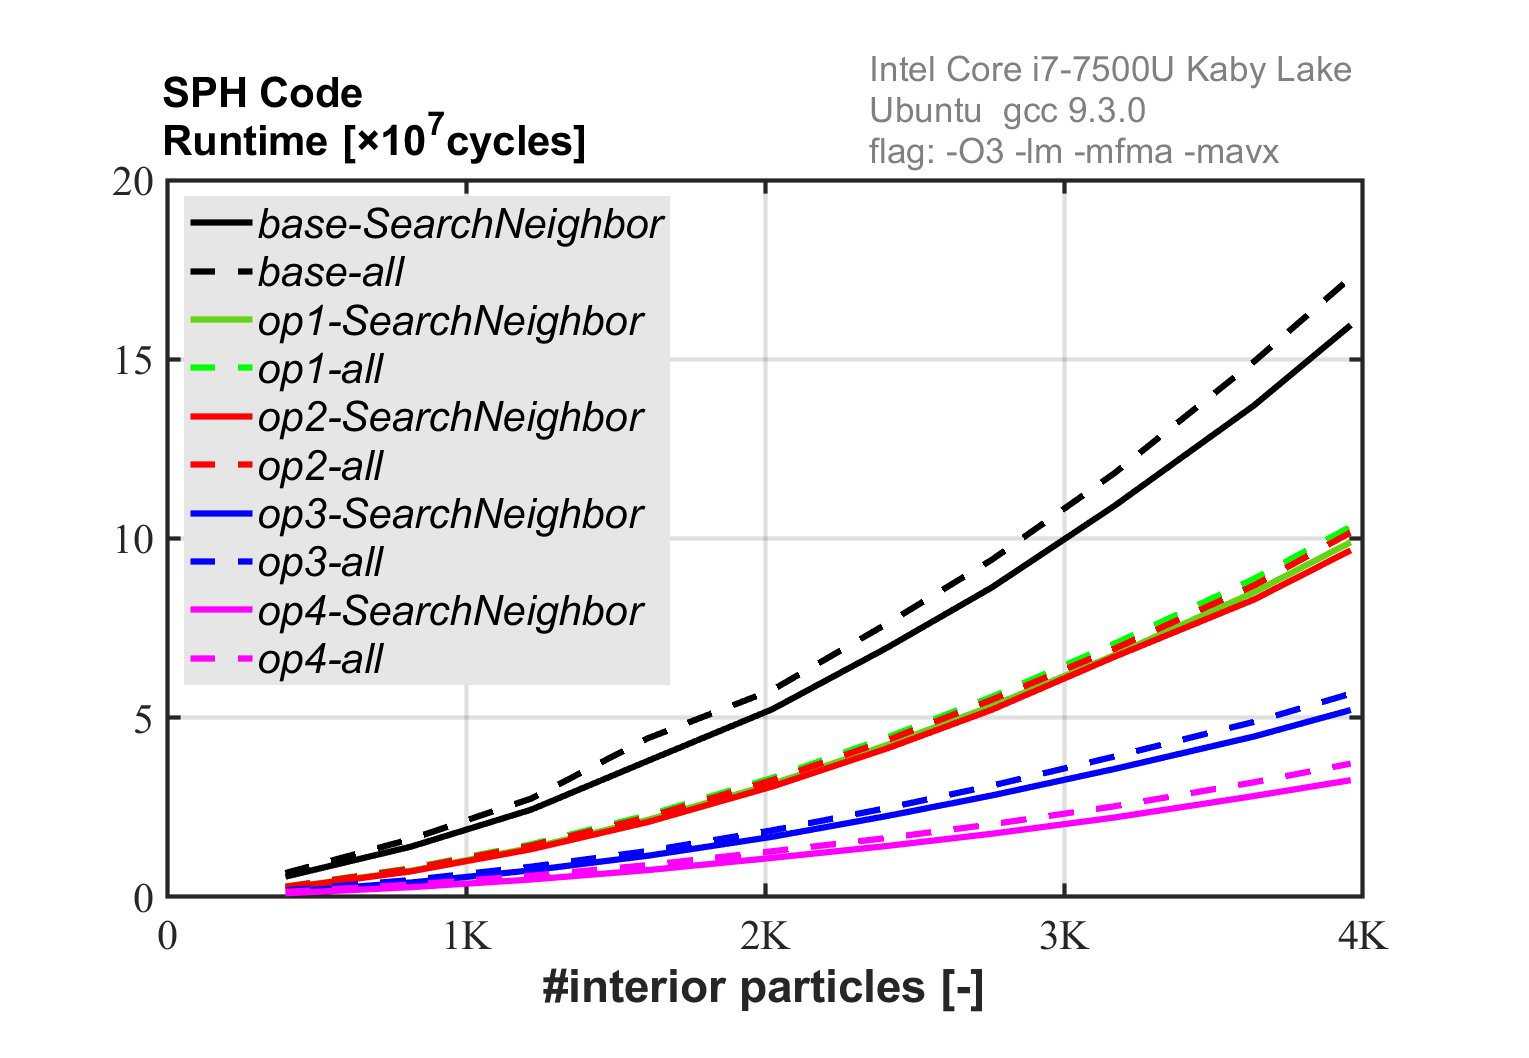
\includegraphics[trim={1.2cm 0.3cm 2.2cm 0.6cm},clip, width=\linewidth]{runtime.eps}
    \caption{Runtime of \emph{SearchNeighbor} and of the whole code for the baseline and for the four optimized versions.}
    \label{fig:runtime}
\end{figure}
The most improvement is for smaller input sizes and decreases for larger ones. 
Whereas for the base version the operational intensity is fluctuating around values below one, the operational intensity of optimization 1 is constantly increasing for ascending input size (see Fig. \ref{fig:roofline}).
\begin{figure}
    \centering
    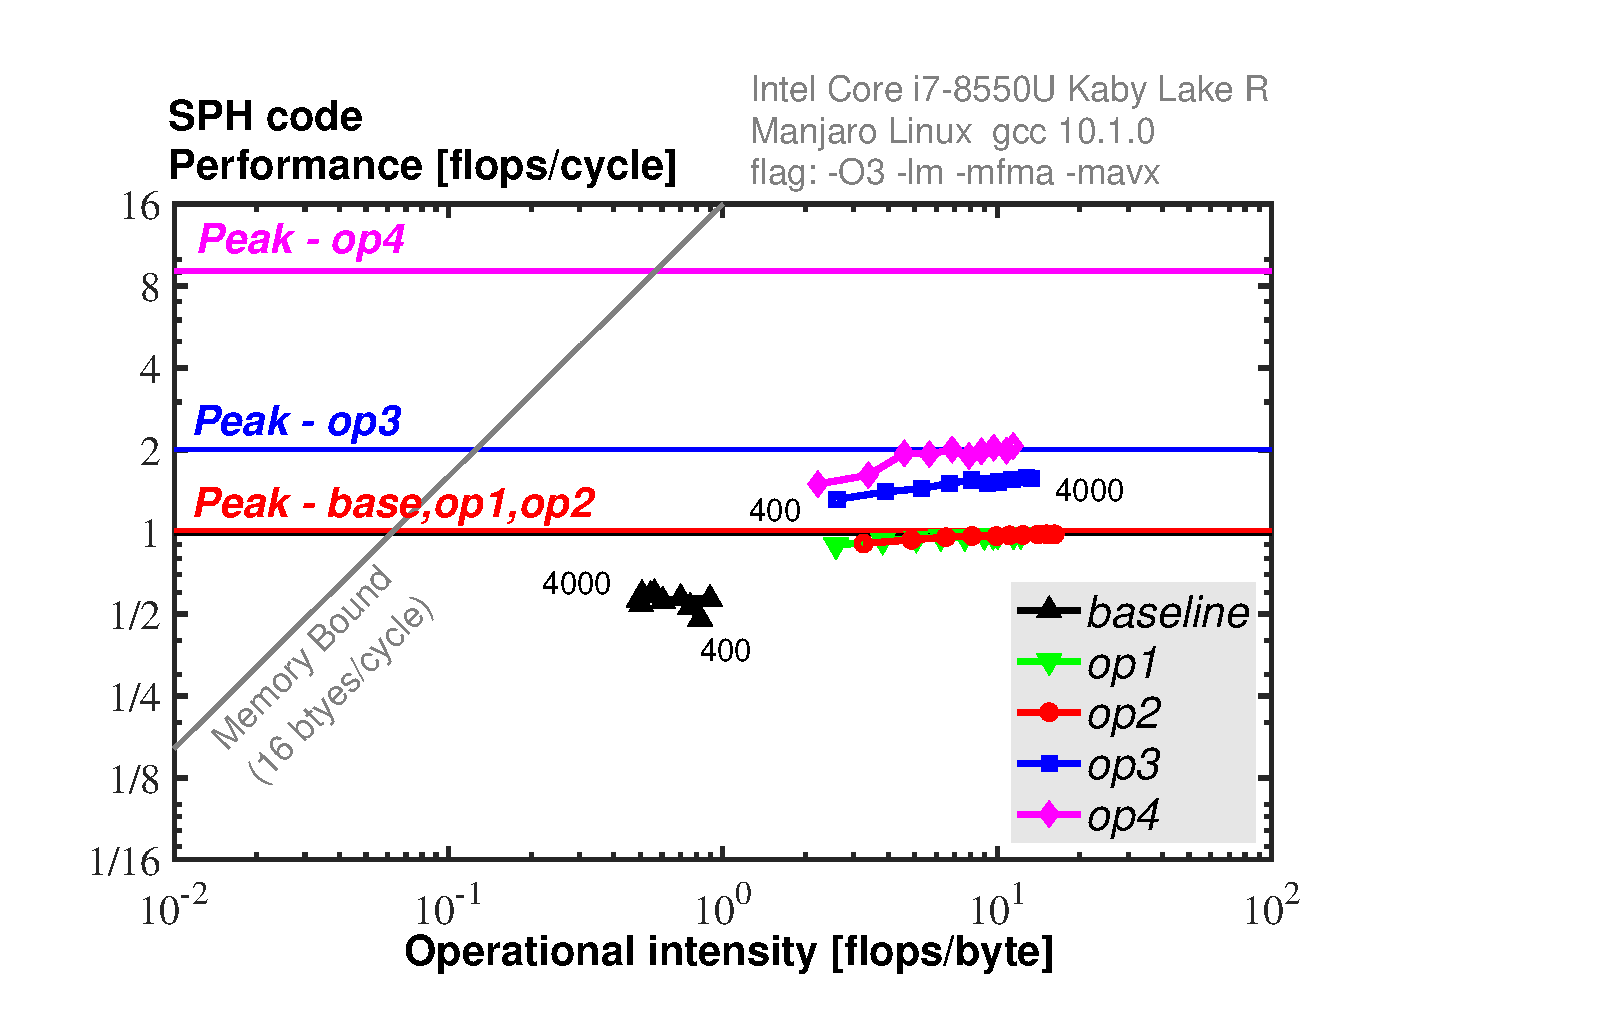
\includegraphics[trim={1.2cm 0.3cm 2.2cm 0.9cm},clip, width=\linewidth]{roofline.eps}
    \caption{Roofline plot of all the functions in the baseline and the four optimized versions. There is only a small variation ($\pm 9\%$) in the flop operations count.}
    \label{fig:roofline}
\end{figure}
The same applies also for the performance of these versions.
Nevertheless, the performance and even more the operational intensity is improved considerably by the first optimization part. 
This is primarily attributed to the changed data structure. 
A minor part is also due to scalar replacement, which is reducing the floating point operations slightly.

%op2: blocking and unrolling
After applying the second portion of optimization (\emph{optimization 2}), the performance almost stays where it was.
On the other side the operational intensity is improved by implementing the blocking and unrolling. 
With a closer look at the stores and loads, which are causing this improvement, it is evident that the key improvement is due to reduced last-level cache stores.
At the same instant the floating point operations are the same for the first optimization part and the second one. 
It seems that this optimization part is not really worth it.
The main reason for that is the significant overhead introduced with this optimization to treat each remainder part of the factors used for blocking and unrolling.
The reasoning behind this fact is that our setup does not allow us to choose arbitrary numbers for inputs size. Based on the input the closest possible value that satisfies the configuration of the simulation is taken.
Therefore, it is impossible to require any assumption about divisibility of the input size by a certain factor.
As a result the code has to be written in a general way to handle each input size correctly.
Conclusively, this leads to only a small improve on the operational intensity for unrolling and blocking.

%op3: vectorization and AoS to separate arrays for vector type
The performance from the second to the third optimization part (\emph{optimization 3}) rises by a factor of somewhat below two.
However, the operational intensity diminishes back to the values of optimization part one.
This deterioration comes from the increase of last-level cache stores of the neighbors.
A cause of this is most likely the increase of the unrolling factor by a factor of four.
Hence, there are sixteen consecutive \emph{if} statements for the lines 7 and 16 in Algorithm \ref{algor:searchneighbor_op_1}, after which the storing of the neighbors is done if the condition is satisfied.

%op4: postpone sqrt and compare with squared H
In the next and ultimate step of the optimization process (\emph{optimization 4}) we reduced the floating point operations by approximately fifteen percent by computing less square root functions. This reduces the overall run-time by a further third with respect to the third optimization part as seen in Fig. \ref{fig:runtime}. Furthermore, this implementation with all the optimizations done is four and a half times faster than our base one. 
In addition, the operational intensity as shown in Figure \ref{fig:roofline} decreases together with the floating point operations compared to the other optimized versions.

%PEAK performance:
To sum up, the performance of the code has more than quadrupled after applying the different optimization steps.
In comparison with the computed peak performance of around nine flops per cycle for the final version the best performance of around two is comparatively small.
In addition, the performance increases with the input size for all optimized versions.

%memory und compute bound
As it is shown in Figure \ref{fig:roofline} our code lies always in the compute bounded region for the different version of it. Due to that the memory bandwidth of 16 bytes/cycle has no major impact on the code, but rather the peak performance has.

The theoretical peak performance of the different versions is computed according to the cost measure stated in Equation \ref{eq-4} with consideration of the throughput of the various operations.
Even though there is some auto-vectorization of the compiler, the peak performance is computed considering only vectorization where explicitly used (i.e. \emph{optimization 3 and 4}).
The reasoning behind this fact is that the major part of \emph{SearchNeighbor} is not auto-vectorized.
In short the theoretical peak performance is calculated based on a rather limited optimization: not considering the compilers auto-vectorization. 
Consequently, the performance of the first and second optimization part is close to their scalar peak performance.
On the contrary, the performance diverges more from its peak performance for the third optimization part and even more for the fourth one.
The peak performance of \emph{optimization 3} is dominated by the square root functions with lower throughput for the vectorized operation.
Because of this the peak performance is not quadrupled compared to the scalar one.
However, the peak performance for the fourth version is increased significantly for the considerably fewer number of square root function with a tiny throughput.

%Compiler flags
Having this improvement, the run-time can be reduced by a few percent by using the clang compiler. Moreover, the additional flags \emph{-ffast-math} and \emph{-march=native} reduced the run-time for both compilers (gcc, clang). With the use of profiling flags for the different compilers, the run-time decreased a little bit further. Interestingly, the clang compiler optimized the base version of our code worse than gcc.

%------------------------------------------------------------------------------------------------------
\section{Conclusions}\label{sec:conclusions}
By applying the different optimizations, we achieved a speedup of roughly 5x on a single-core. 
The most valuable optimizations were the changing of the data structure with the involved branch reduction, vectorization and the reduction of the square root computations. Note that our optimizations are highly case- and architecture-dependent and may come at the cost of generality and code readability.

According to our analysis, it is hard to get further significant improvement based on the final optimization without modifying the algorithm. Because of the nature of neighboring search algorithm, it is impossible to get rid of branches and it is hard to vectorize them, which slow down the simulation tremendously. Although other parts of the simulation can still be improved, they would not deliver any remarkable speedup, since less then ten percent of the run-time is consumed by them. However, we suppose that by initializing particles in a smarter way, we may achieve additional improvement. Currently, all the particles are initialized row-wise or column-wise. It would make sense to initialize them block-wise, such that particles that are close to each other in the space are also close in memory.

Even so, the way how we optimize searching neighbors can be widely used for similar simulators, and even applicable in other fields.
%-8 pages till here --------------------------------------------------------------------------------------
\section{Contributions of Team Members}
Note that for all the optimizations all of us tried to implement them and we picked only the best version of them (faster in terms of cycles and smarter version).
Also, we implemented the code from scratch, and this required us a lot of work. In particular, getting a working SPH simulator for our configuration was very time-consuming.

\mypar{Silvia} 
Base version: implementation of the pressure, the speed of sound, the initialization of the particles together with Valérie and the movement of the boundaries. Validation of the code. 
Code optimizations: vectorization (optimization 3) and postponing of the sqrt (optimization 4). Analysis of the results: cost analysis and computation of the peak performance. General analysis of the results.

\mypar{Mengdi}
For baseline implementation: implementing time integration.
For optimization 1: changing data structure, function inling. 
For optimization 2: implementing and testing unrolling and blocking separately, and combing them.
For optimization 3: determining unrolling factor and block size. 
For all implementations and plots: data measurement and analysis.

\mypar{Tianwei}
For baseline, implementing basic data structure, kernel related functions, neighbor search and viscose term;
For optimization, do branch reduction; participate in blocking; participate in vectorization; make plots.

\mypar{Valérie} Implemented the computation of the acceleration. Done Scalar replacement. Computation of interior and boundary particles and smoothing length with input given and adapting initialization of simulation with Silvia. Implemented a own variant of unrolling and vectorization. First cost analysis of code. Tried different compiler and flags. Took measurements for roofline plot with perf and analysed them.

% References should be produced using the bibtex program from suitable
% BiBTeX files (here: bibl_conf). The IEEEbib.bst bibliography
% style file from IEEE produces unsorted bibliography list.
% -------------------------------------------------------------------------
\bibliographystyle{IEEEbib}
\bibliography{bibl_conf}

\end{document}